\documentclass{article}
\usepackage{graphicx}
\usepackage{epsfig}
\title{Gedistribueerde systemen chatserver}
\author{Victor Azizi \\ azizivictor@gmail.com \\ studentnummer 6277861}
\date{\today}
\begin{document}
\section{Inleiding}
In dit verslag leg ik uit hoe ik de chatserver voor het vak gedistribueerde systemen heb geschreven. Ik zal beginnen met het uitleggen van het oorspronkelijke plan en de daarbij behorende keuzes, waarna ik doorga met uitleggen hoe het werkelijk is gegaan en welke keuzes ik daarbij heb gemaakt. Daarna zal ik het resultaat beschrijven met alle features die het programma wel en/of niet heeft. Als laatste ga ik de chatserver terugkoppelen aan de oorspronkelijke opdracht en kijken hoe dat is gegaan en ook beargumenteren wat er goed is gegaan en wat er beter had gekund.
\section{Plan van aanpak}
\begin{figure}[htb]
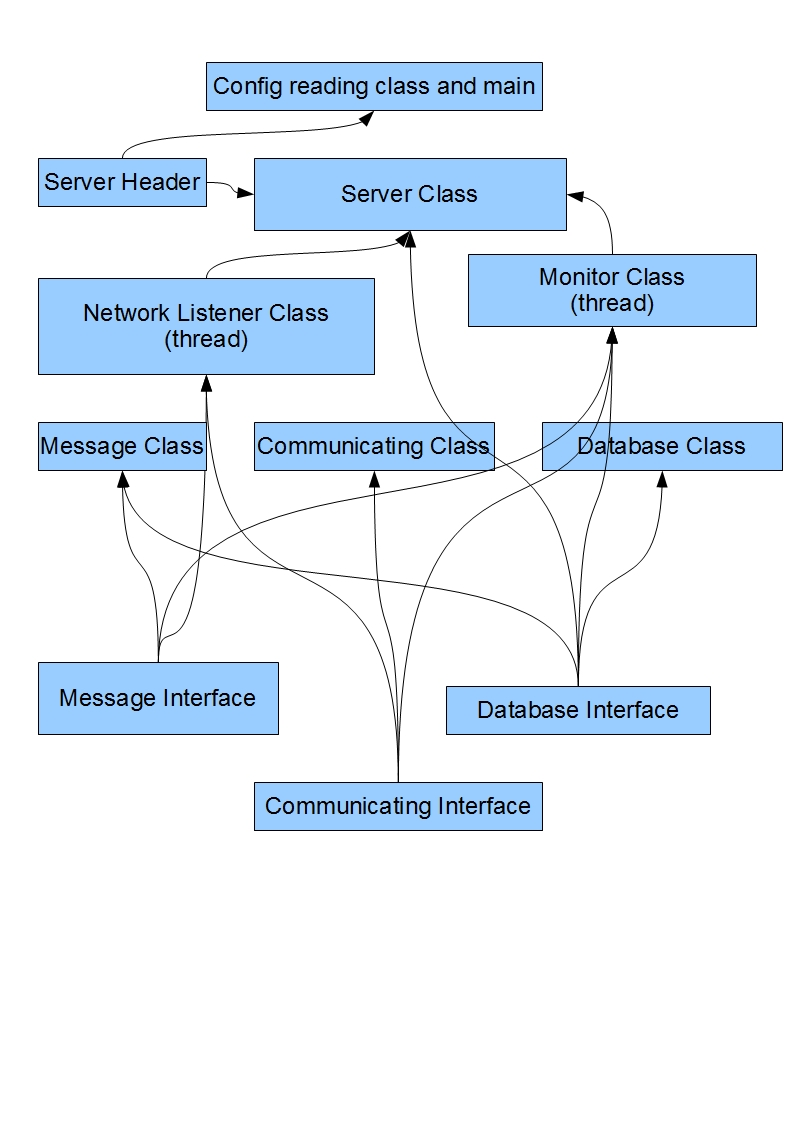
\includegraphics[trim = 0mm 100mm 0mm 0mm, scale=0.3]{doc/Flowchart.jpg}
\caption{Een visueel concept van de chatserver} 
\end{figure}
De taal die ik ga gebruiken is C++ om de volgende redenen:
\begin{itemize}
\item Goeie libraries voor internet communicatie.
\item Met behulp van Object oriented programming is het mogelijk het geheel een stuk leesbaarder en overzichterlijker te maken.
\item Standaard beveiliging (Buffer overflow etc) al ingebouwd.
\end{itemize}
De keuze voor het versiebeheersysteem is is op git gevallen. Dit omdat het makkelijk en snel in gebruik is in tegenstelling tot andere versiebeheersystemen.
\newline
\subsection{Regels voor de chatserver}
\begin{itemize}
\item Ping en Timeout
\begin{itemize}
\item Stuur elke 5 seconden een ping naar alle instanties waar je mee verbonden bent
\item Als je 15 seconden lang geen antwoord krijgt van een verbonden instantie dan mag je de verbinding verbreken
\begin{itemize}
\item Is deze instantie de parent-server vraag dan ook een nieuwe parentserver aan de controlserver
\end{itemize}
\item Als je 35 seconden niks hebt gehoord van de controlserver ben je uit het netwerk gehaald. Probeer opnieuw te verbinden.
\end{itemize}
\item Berichten
\begin{itemize}
\item Kijk of de afzender bevoegd is om dit bericht te sturen
\item Controleer of het een valide bericht is
\item Reageer zoals wordt verwacht
\end{itemize}
\item Database
\begin{itemize}
\item De database moet per verbinding alle informatie hierover bijhouden in een entry
\end{itemize}
\item Structuur
\begin{itemize}
\item De onderdelen van het programma moeten los van elkaar te gebruiken zijn, dit betekent dat de database of andere onderdelen makkelijk te vervangen/hergebruiken moeten zijn.
\end{itemize}
\end{itemize}
\section{Uitwerking}
Ik ben begonnen met het maken van een framework voor de chatserver.
Dit heb ik gedaan door aan de hand van het visuele concept header files te schrijven met daarin elk aparte classes.
Deze files zijn te vinden in de headers directory.
Nadat ik deze had geschreven ben ik ze gaan implementeren, te beginnen met connection, message en database.
Daarna heb ik deze bij elkaar gebracht in de server.
Toen bleek dat de database niet goed genoeg was omdat hij te weinig informatie opsloeg.
Hij maakte namelijk geen verschil in direct en indirect verbonden clients.
Gelukkig was de class zelf al wel redelijk goed beschreven en was het slechts een kwestie van herschrijven voordat deze het goed deed.
Ik heb in de server class een functie geschreven die al het binnenkomende verkeer afhandeld.
Door per bericht te kijken in welke staat de server zich bevind kan worden bepaald hoe er geantwoord moet worden, dit is eigenlijk een groot switch-case statement.
Hierna heb ik met behulp van select() (een functie die wacht op input in combinatie met een timeout) een monitor algorithme gemaakt.
Deze monitor checkt elke 5 seconden of een client inactief is en/of verwijderd moet worden.
Toen dit goed werkte heb ik als laatste de manager functionaliteit toegevoegd.
Omdat ik weinig tijd had hiervoor heb ik het niet mooi objective oriented geimplementeerd maar als if-statements in incomingmessage.cpp
\section{Resultaat}
Het resultaat is een zeer stabiele en snelle server met een kleine memory-footprint na het opstarten (1.1KB). 
De manager functionaliteit is ondanks tijdgebrek bijna volledig geimplementeerd.
Het is alleen niet mogelijk om van een niet manager nickname je naam te veranderen naar die van de manager. 
Gelukkig is dit slechts een klein ongemak, en werkt de rest wel.
Uit de gezamelijke tests blijkt ook dat de server goed werkt en compitabel is met de andere servers want niemand heeft de verbinding met mijn server verbroken en hij was na een tijdje de hele tijd root van het netwerk.
Ook lukte het om berichten van en naar andere servers te sturen.
\section{Discussie}
Men kan zeggen dat de server werkt naar behoren en volgens het protol omdat hij goed samen kan werken met andere servers.
Uit die testen bleek namelijk ook dat dit niet altijd zo hoeft te zijn.
De afwerking van het geheel had wat beter gekund (duidelijkere logs, nog betere structuur), al is dat nu niet heel rampzalig.
\end{document}
